%%%%%%%%%%%%%%%%%%%%%%%%%%%%%%%%%%%%%%%%%%%%%%%%%%%%%%%%%%%%%%%%%%%%%%%
%%%                           System Description
%%%%%%%%%%%%%%%%%%%%%%%%%%%%%%%%%%%%%%%%%%%%%%%%%%%%%%%%%%%%%%%%%%%%%%




\chapter{Discussion}
We designed and implemented a role-playing game that puts the player as an attacker and shows different phishing techniques attackers can use.  Overall, we are pleased with the result of this first iteration of the game and its ability to convey educational materials.

\section{Insights}
We noticed a few common patterns during our study, and we believe additional training materials on these would help strengthen users against phishing attackers.

\subsection{Mailing Domains and Subdomains}
Legitimate emails used in our survey used "info@mailer.netflix.com" as the sender, which is the email used by Netflix to send updates about user accounts. We noticed that participants marked these legitimate emails "Maybe phishing" or "phishing" although they were satisfied with other contents of the email.

We believe the confusion is mainly due to the following two reasons:

\begin{enumerate}
    \item Users are expecting the email to be from netflix.com. However, confusion arises when users see emails originate from "mailer.netflix.com." We can see a similar example in figure \ref{fig:lyft}. Lyft used "noreply@lyftmail.com" to send the email. This pattern can easily confuse users, and attackers can potentially use similar patterns for other organizations to trick the victims.

    \item The issue mentioned in (1) also highlights another problem with current phishing training modules: subdomains. Although our game touches it briefly (and many games discussed in the literature review briefly cover it), we haven't found games that fully cover subdomains.
\end{enumerate}

\begin{figure}
    \centering
    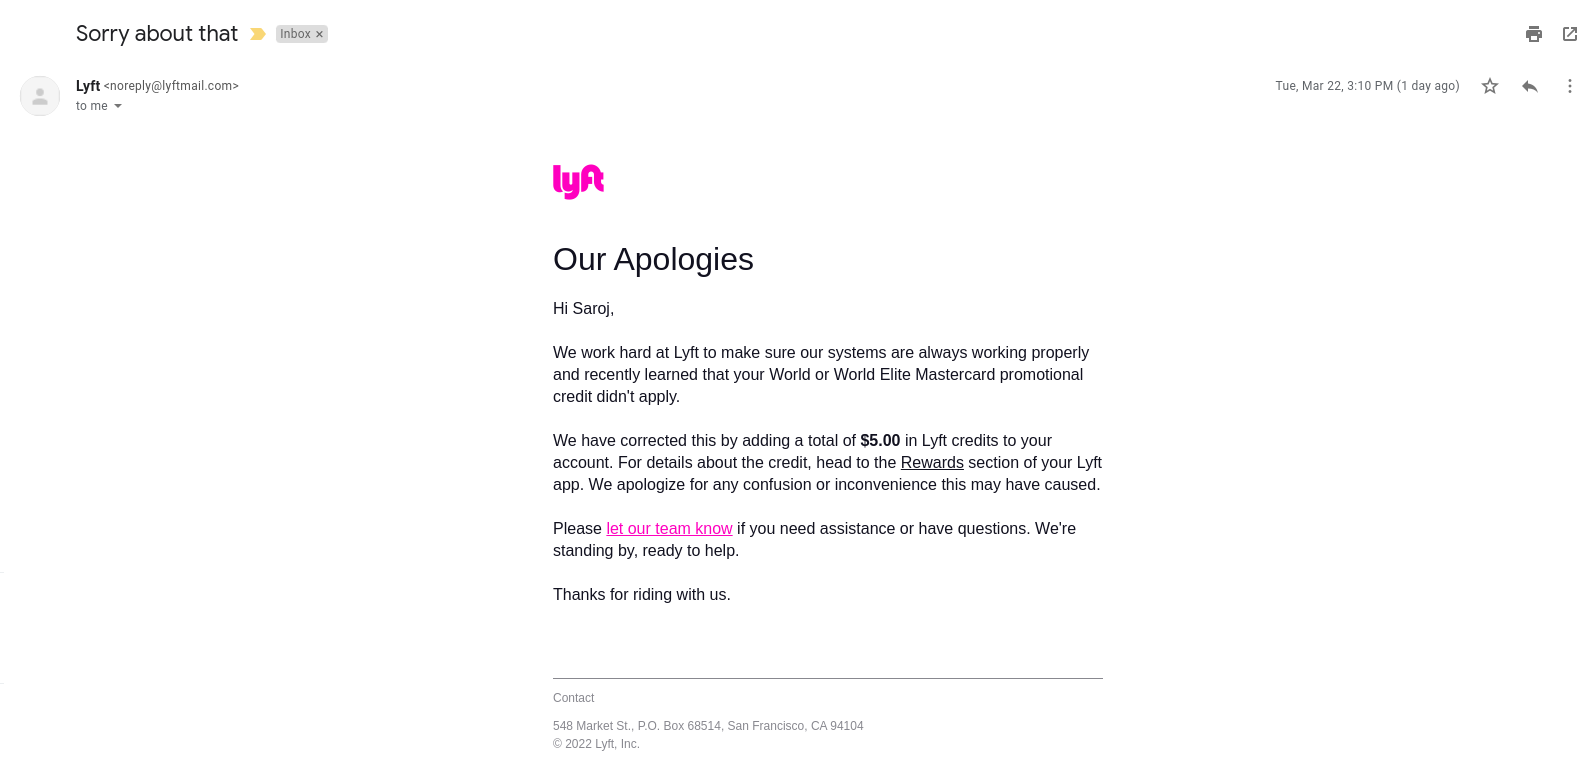
\includegraphics[width=\textwidth]{section4/lyft.png}
    \caption[An email sent by Lyft]{An email sent by Lyft. The sender of the email is \textit{noreply@lyftmail.com}}
    \label{fig:lyft}
\end{figure}

We can mitigate this problem if organizations (such as Netflix) warn the users about the domains they use or stick with a similar pattern of domains when emailing the user. In addition, new games should focus on developing games that include subdomains as a seperate training module instead of incorporating it inside link training.

\subsection{Issues with email content}
Our pre-survey (and in some part post-survey) showed participants did not like when they got personal information (such as phone number and credit card number) in their email. We believe users would be more comfortable with such emails if they only notified the user of changes through emails and gave the details in their platform.

\section{Limitations and Future works}
We conducted a user study with 11 participants, which provided important insight into the game's viability, but further studies are needed to confirm that the results hold in other settings. In addition, most of our participants had some previous knowledge about phishing. Therefore, we need to further study with diverse demographics to verify the works even when participants have no prior knowledge. Furthermore, the interpretation of players' comments may have been biased by our intimate knowledge of the game, although we made every effort to remain objective.

The overall experience of our gameplay takes around 25 minutes. We can incorporate larger demographics by creating a compact version of the game. Based on the feedback, participants were willing to share the game with friends and family if it required a shorter time commitment.

The current iteration of the game does not focus on subdomains. However, our results show that subdomain is an area that requires more focus. Future improvements can be made by adding subdomains as a separate training module.
% \section{Future Work}
% We want to create a compact version of the game. Users would happily share the game with friends and family if it were shorter based on the comments.


\section{Conclusion}
We designed and developed a role-playing game that lets the player play as an attacker and explore different phishing techniques attackers can use. The main goal of our games is to teach players anti-phishing techniques by showing the players different tricks attackers. We conducted our user study with 11 participants and presented our results demonstrating our game positively impacted players' confidence to detect phishing emails. In addition, we listed a few common patterns that we found during our study. Based on the result, we found some areas such as subdomain and organization emails that require more focus.

Overall, we are pleased with the result of this first iteration of the game and its ability to convey educational materials. This game can serve as a good starting point for future work.